\hypertarget{proluxe9taires-de-tous-les-pays-unissez-vous}{%
\section{Prolétaires de tous les pays, unissez-vous
!}\label{proluxe9taires-de-tous-les-pays-unissez-vous}}

\emph{Dimanche 27 mai 2018}

Bonsoir à tous !

Nous sommes arrivés à Moscou vendredi.

Nous avons eu droit à un accueil formidable de la part de nos deux hôtes
russes, Stanislav et Irma, et nous sommes déjà largement promenés dans
le centre-ville de Moscou.

\begin{figure}
\centering
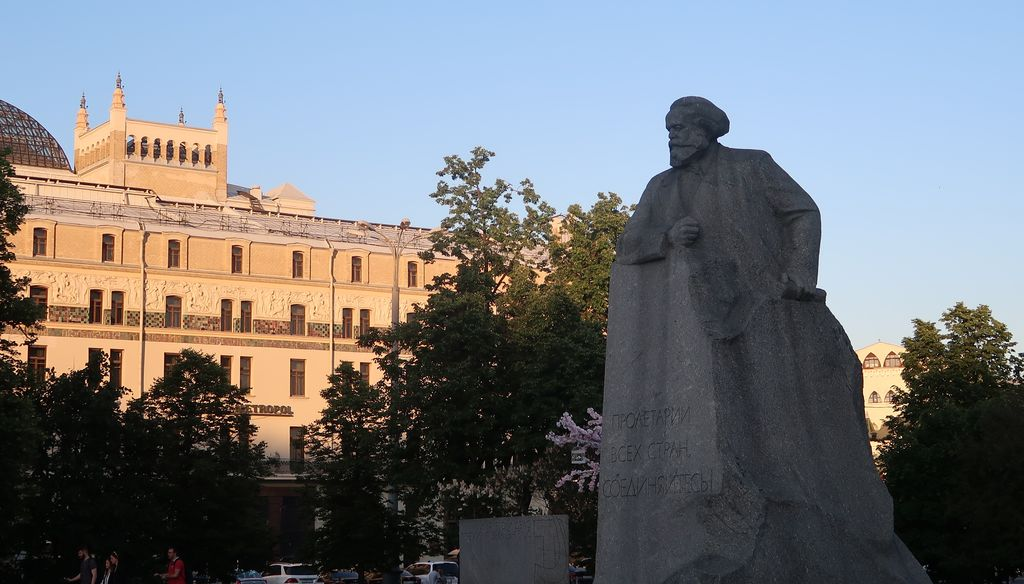
\includegraphics{images/20180527_marx.JPG}
\caption{La statue de Marx près de la place Rouge, sur le socle de
laquelle il est écrit "Prolétaires de tous les pays, unissez-vous !". Un
slogan aujourd'hui étonnant, caché en plein centre-ville.}
\end{figure}

Alors que dire, à ce stade, de nos impressions ? Je suis sous le charme
de la grande et belle ville de Moscou. Et en même temps, un mystère
demeure : c'est donc ici, le pays de Vladimir Poutine et de l'ancienne
URSS ? Mes idées reçues ne correspondent pas à la soirée quasi-estivale
que nous venons de passer avec ces groupes qui font de la musique en
plein-air et tout ce beau monde qui se promène.

Affaire à suivre !

\emph{Florian}

\hypertarget{commentaires}{%
\subsection{Commentaires}\label{commentaires}}

\begin{itemize}
\item
  Thibaud, \emph{2018-05-29 19h08}

  Dis-toi que bientôt des milliers de fan de foot vont se dire
  exactement la même chose \^{}\^{} Ce qui est très bon pour la Russie.
  Perso ça me fait plaisir !
\item
  pythux, \emph{2018-05-31 10h18}

  Pourquoi les fans de foot se diraient "prolétaires unissez-vous" ? :p
  Le foot n'intéresse pas que les prolétaires !!
\item
  Thibaud, \emph{2018-06-25 20h40}

  On voit les mecs qui ne lisent que le titre avant de filer aux
  commentaires \^{}\^{}
\item
  pythux, \emph{2018-06-25 20h44}

  Le contenu de l'article n'est qu'on prétexte ! Les commentaires, c'est
  là que tout se passe !
\item
  pythux, \emph{2018-05-31 10h25}

  On ne m'ôtera pas de l'idée, que tout ceci date de l'époque où ils
  con-solidaient une certaine idéologie en con-struisant des statues
  partout. La fameuse con-stellation de la grande URSS.
\end{itemize}
